\documentclass[11pt, oneside]{article} 
\usepackage{geometry}
\geometry{letterpaper} 
\usepackage{graphicx}
	
\usepackage{amssymb}
\usepackage{amsmath}
\usepackage{parskip}
\usepackage{color}
\usepackage{hyperref}

\graphicspath{{/Users/telliott_admin/Tex/png/}}
% \begin{center} 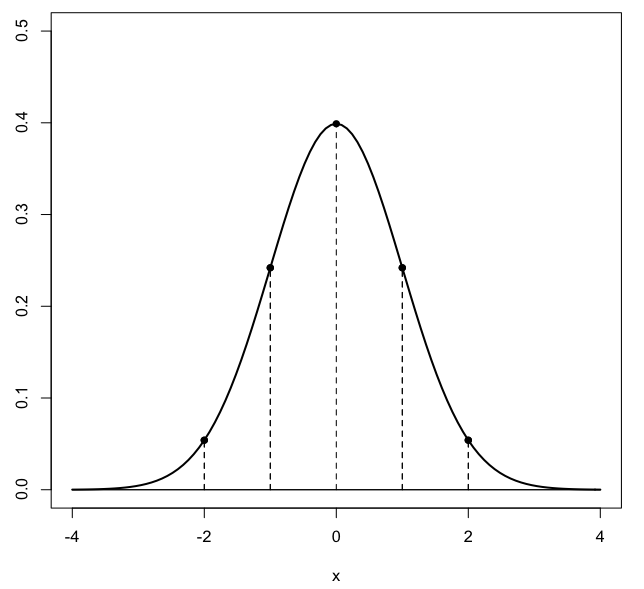
\includegraphics [scale=0.4] {gauss3.png} \end{center}

\title{Complex function theory}
\date{}

\begin{document}
\maketitle
\Large

One motivation for learning about complex functions is that the theory is often described as being very beautiful.  It also shows how certain more difficult integrals can be solved. 

Marsden gives three examples that he says are either very difficult or impossible if we are restricted to just the real numbers:

\[ \int_0^{\infty} \frac{\sin^2 x}{x^2} \ dx = \frac{\pi}{2} \]
\[ \int_0^{\infty} \frac{x^{\alpha - 1}}{1 + x} \ dx = \frac{\pi}{\sin \alpha \pi} \]
\[ \int_0^{2 \pi} \frac{1}{a + \sin \theta} \ d \theta = \frac{2 \pi}{\sqrt{a^2 - 1}} \]

Here's another from Nahin.
\[ \int_{-\infty}^{\infty} \frac{\cos x}{1 + x^2} \ dx = \frac{\pi}{e} \]


Maybe we can learn to solve these before we're done.


\end{document} 